% Speaker build with notes on a second screen.
\documentclass[aspectratio=169,11pt]{beamer}
% Shared preamble for the agents-analog-digital tutorial.
% Mirrors tutorials/rtl2gds-gf180-docker/preamble.tex so both decks
% look identical.

\usetheme{metropolis}
\setbeamertemplate{footline}[frame number]
\setbeamertemplate{navigation symbols}{}

\usepackage[T1]{fontenc}
\usepackage[utf8]{inputenc}
\usepackage{lmodern}
\usepackage{graphicx}
\usepackage{booktabs}
\usepackage{array}
\usepackage{xcolor}
\usepackage{listings}
\usepackage{tikz}
\usepackage{hyperref}
\usepackage{fancyvrb}
\usepackage{pgfpages}

\usetikzlibrary{arrows.meta,positioning,shapes.geometric,fit,backgrounds,
                calc,decorations.pathreplacing,shadows}

\definecolor{accent}{HTML}{2B6CB0}
\definecolor{accent2}{HTML}{2F855A}
\definecolor{accent3}{HTML}{C05621}
\definecolor{muted}{HTML}{4A5568}
\definecolor{softbg}{HTML}{F7FAFC}
\definecolor{codekw}{HTML}{805AD5}
\definecolor{codestr}{HTML}{2F855A}
\definecolor{codecom}{HTML}{718096}

\lstdefinestyle{shellstyle}{
  language=bash,
  basicstyle=\ttfamily\scriptsize,
  keywordstyle=\color{codekw}\bfseries,
  commentstyle=\color{codecom}\itshape,
  stringstyle=\color{codestr},
  backgroundcolor=\color{softbg},
  frame=single,
  rulecolor=\color{muted!40},
  showstringspaces=false,
  breaklines=true,
  columns=fullflexible,
  keepspaces=true,
  literate={~}{{\textasciitilde}}1 {\$}{{\$}}1 {-}{{-}}1,
}
\lstset{style=shellstyle}

\newcommand{\term}[1]{\textbf{\color{accent}#1}}
\newcommand{\cmd}[1]{\texttt{\small#1}}
\newcommand{\warn}[1]{\textbf{\color{accent3}#1}}

\tikzset{
  agent/.style={
    draw=accent, thick, rounded corners=2pt, fill=accent!8,
    minimum width=2.6cm, minimum height=0.9cm, align=center, font=\small
  },
  agent2/.style={
    draw=accent2, thick, rounded corners=2pt, fill=accent2!10,
    minimum width=2.6cm, minimum height=0.9cm, align=center, font=\small
  },
  agent3/.style={
    draw=accent3, thick, rounded corners=2pt, fill=accent3!10,
    minimum width=2.6cm, minimum height=0.9cm, align=center, font=\small
  },
  arrow/.style={-Stealth, thick, accent!80},
  arrow2/.style={-Stealth, thick, accent2!80},
}

\setbeameroption{show notes on second screen=right}

\title{AI Agents for Analog and Digital IC Design}
\subtitle{What the eda-agents stack actually ships today}
\author{EDA-Agents Project}
\institute{Open-Source IC Design}
\date{\today}

\begin{document}

\begin{frame}[plain]
  \titlepage
\end{frame}

\begin{frame}{What you will learn}
  \begin{itemize}
    \item How the \cmd{eda-agents} repo splits AI assistance into two
          loops: analog (sizing + SPICE) and digital (RTL-to-GDS).
    \item The roster of agents and the infra they plug into.
    \item Where to go to drive a real block end-to-end.
  \end{itemize}
  \note{Speaker build: notes shown on the right-hand screen.}
\end{frame}

\begin{frame}{Agenda}
  \tableofcontents
\end{frame}

\section{The landscape}

\begin{frame}{Two design loops, one pattern}
  \begin{columns}[T,onlytextwidth]
    \column{0.48\textwidth}
      \textbf{Analog loop}\\[0.3em]
      \begin{itemize}\small
        \item \term{Inputs}: spec (GBW, PM, noise), topology choice.
        \item \term{Evaluator}: ngspice + gm/ID LUTs.
        \item \term{Knobs}: W/L, bias current, mirror ratios.
        \item \term{FoM}: meets spec? area? power?
      \end{itemize}
    \column{0.48\textwidth}
      \textbf{Digital loop}\\[0.3em]
      \begin{itemize}\small
        \item \term{Inputs}: RTL, clock, die budget.
        \item \term{Evaluator}: LibreLane (Yosys + OpenROAD + KLayout).
        \item \term{Knobs}: density, clock period, PDN pitch.
        \item \term{FoM}: timing slack, area, power, DRC/LVS green.
      \end{itemize}
  \end{columns}
  \vspace{0.8em}
  \begin{center}
    \textit{Both loops share the pattern: propose $\rightarrow$ simulate
    $\rightarrow$ score $\rightarrow$ repeat. The \cmd{eda-agents} repo
    implements it twice, with the same autoresearch core.}
  \end{center}
  \note{%
    Core thesis. Analog and digital feel like different worlds -- one is
    Verilog and flows, the other is W/L ratios and SPICE. But at the
    agent level they are structurally identical: a proposal engine (the
    LLM) emits candidate parameter sets, an evaluator measures them, a
    FoM turns those measurements into a scalar, and a loop repeats.\par
    What differs is the per-evaluation cost. Analog: seconds (ngspice on
    a few transistors). Digital: minutes (LibreLane through routing +
    signoff). The budgets we spend and the search strategies we pick
    follow from that asymmetry.}
\end{frame}

\begin{frame}{What \cmd{eda-agents} ships today}
  \begin{center}
  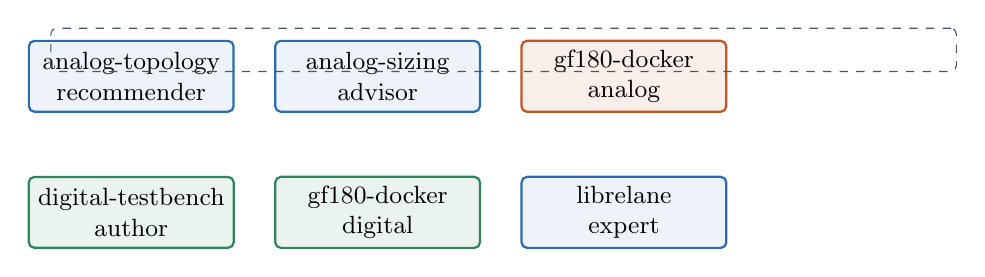
\begin{tikzpicture}[node distance=0.5cm]
    \node[agent] (atr)  {analog-topology\\recommender};
    \node[agent, right=of atr] (asa) {analog-sizing\\advisor};
    \node[agent3, right=of asa] (gfa) {gf180-docker\\analog};
    \node[agent2, below=0.8cm of atr] (dtb) {digital-testbench\\author};
    \node[agent2, right=of dtb] (gfd) {gf180-docker\\digital};
    \node[agent, right=of gfd] (llx) {librelane\\expert};

    \node[draw=muted, dashed, rounded corners=2pt, font=\scriptsize,
          minimum height=0.55cm, minimum width=11.5cm]
         (mcp) at ($(asa.north)!0.5!(gfd.south) + (1.6cm, 1.2cm)$) {};
  \end{tikzpicture}
  \end{center}
  \vspace{0.2em}
  \footnotesize
  \textbf{Analog agents} (blue): recommend a topology, size it with gm/ID,
  harden on GF180 inside Docker.\\
  \textbf{Digital agents} (green): author cocotb TB, drive RTL-to-GDS on
  GF180 inside Docker.\\
  \textbf{Shared infra} (orange/muted): LibreLane expert + MCP server.
  \note{%
    This diagram names the \emph{real} agents shipped in
    \cmd{.claude/agents/} and \cmd{src/eda\_agents/templates/claude\_agents/}
    as of the current main: \cmd{analog-topology-recommender},
    \cmd{analog-sizing-advisor}, \cmd{digital-testbench-author},
    \cmd{gf180-docker-analog}, \cmd{gf180-docker-digital}. There is also a
    \cmd{librelane-expert} agent that specialises in config.yaml
    authoring.\par
    The dashed box above them is the MCP surface -- \cmd{eda-mcp} exposes
    skill templates, LUT access, and tool runners so any outer Claude
    Code session, or an ADK multi-agent hierarchy, can reuse the same
    primitives. We cover that in Section 5.\par
    Naming convention: \cmd{*-docker-*} agents drive
    \cmd{hpretl/iic-osic-tools} via \cmd{docker exec} and own the
    iteration inside the container. The others are planning / coding
    aids that run on the host.}
\end{frame}

\section{Analog side}

\begin{frame}{Analog flow: topology $\rightarrow$ sizing $\rightarrow$ SPICE}
  \begin{center}
  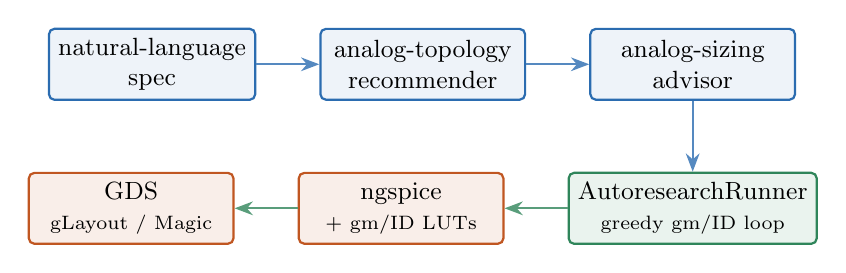
\begin{tikzpicture}[node distance=0.8cm]
    \node[agent]  (nl)  {natural-language\\spec};
    \node[agent, right=of nl]  (rec) {analog-topology\\recommender};
    \node[agent, right=of rec] (adv) {analog-sizing\\advisor};
    \node[agent2, below=0.9cm of adv] (ar)  {AutoresearchRunner\\\scriptsize greedy gm/ID loop};
    \node[agent3, left=of ar] (ng) {ngspice\\\scriptsize + gm/ID LUTs};
    \node[agent3, left=of ng] (gds) {GDS\\\scriptsize gLayout / Magic};

    \draw[arrow]  (nl) -- (rec);
    \draw[arrow]  (rec) -- (adv);
    \draw[arrow]  (adv) -- (ar);
    \draw[arrow2] (ar) -- (ng);
    \draw[arrow2] (ng) -- (gds);
  \end{tikzpicture}
  \end{center}
  \vspace{0.3em}
  \begin{itemize}\footnotesize
    \item \cmd{analog-topology-recommender}: maps a one-line spec
          ("rail-to-rail OTA, 10 MHz GBW") to a registered topology
          (Miller OTA, telescopic, folded cascode, SAR-ADC,\ldots).
    \item \cmd{analog-sizing-advisor}: consumes the chosen topology plus
          gm/ID LUTs; proposes a starting W/L + bias point; hands off to
          \term{AutoresearchRunner} for the SPICE-scored greedy refinement.
    \item \cmd{gf180-docker-analog}: finalises layout + runs DRC/LVS
          inside \cmd{hpretl/iic-osic-tools}.
  \end{itemize}
  \note{%
    The analog loop is where \cmd{eda-agents} has the most depth. The
    methodology is \term{gm/ID}: pre-computed LUTs encode the
    device-level trade-off (transconductance vs current) for each
    transistor type on each PDK. The sizing advisor uses those tables to
    hand the autoresearch runner a good starting point -- not a random
    one -- so the subsequent SPICE budget is spent on refinement, not
    discovery.\par
    Supported circuit topologies today (registered as
    \cmd{CircuitTopology} subclasses under
    \cmd{src/eda\_agents/topologies/}): Miller OTA, AnalogAcademy OTA,
    GF180 OTA, StrongArm comparator, SAR ADC (8b, both transistor-level
    and behavioral variants). Topology-agnostic core means ``add another
    circuit'' is \cmd{\~200} lines of code per topology.\par
    Layout: \cmd{gLayout} (Python-based parametric layout) in a sibling
    venv, Magic for DRC/LVS, KLayout for streamout. The ADK harness
    drives those as sub-agents \cmd{FlowRunner}, \cmd{DRCChecker},
    \cmd{LVSVerifier}.}
\end{frame}

\begin{frame}{Key skills and artefacts -- analog}
  \footnotesize
  \begin{tabular}{@{}p{0.40\textwidth}p{0.55\textwidth}@{}}
    \toprule
    \textbf{Asset} & \textbf{What it does} \\
    \midrule
    \cmd{analog.gmid\_sizing} skill & Prompt template + policy for gm/ID
        starting-point selection. \\
    \cmd{analog.explorer} skill & Proposes next-step sizing moves; reads
        \cmd{program.md} and \cmd{results.tsv}. \\
    \cmd{analog.corner\_validator} & Re-runs the best candidate across
        PVT corners before accepting. \\
    \cmd{analog.behavioral\_primitives} & Catalogue of XSPICE + Verilog-A
        primitives (ideal comp, clock gen, sampler) for top-down SAR,
        PLL, LDO blocks. \\
    \cmd{analog.sar\_adc\_design} & End-to-end SAR ADC skill (8b-11b;
        references \cmd{sar\_adc\_8bit\_behavioral} topology). \\
    \midrule
    \cmd{AutoresearchRunner}
        (\cmd{src/.../autoresearch\_runner.py}) & The greedy loop.
        Persists \cmd{program.md} (narrative) + \cmd{results.tsv} for
        resumable runs. \\
    \cmd{SpiceRunner}
        (\cmd{src/.../spice\_runner.py}) & Sync + async ngspice with
        measurement parsing. \\
    \bottomrule
  \end{tabular}
  \note{%
    All the skill names are dotted namespace entries registered in
    \cmd{src/eda\_agents/skills/analog.py}. The MCP server exports them
    so any agent (ours or a user's) can request the prompt by name
    rather than copy-pasting text.\par
    The \cmd{program.md} + \cmd{results.tsv} pair is a Karpathy-style
    autoresearch trace: the LLM reads its own prior thinking and
    measurements, making runs \emph{resumable}. That is how we handle
    10+ hour budgets without blowing context windows.}
\end{frame}

\section{Digital side}

\begin{frame}{Digital flow: master agent + four specialists}
  \begin{center}
  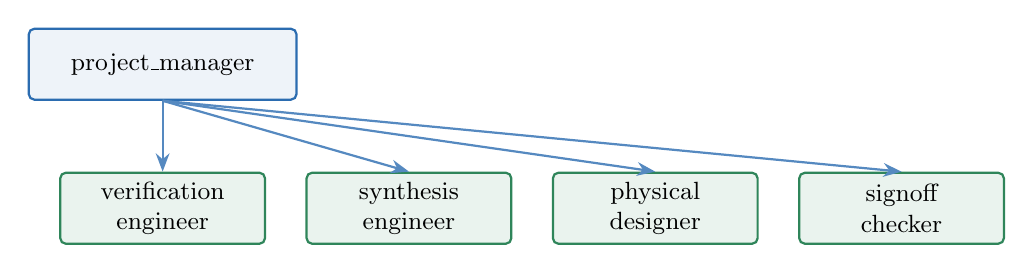
\begin{tikzpicture}[node distance=0.4cm and 0.5cm]
    \node[agent, minimum width=3.4cm] (pm) {project\_manager};
    \node[agent2, below=0.9cm of pm] (ve) {verification\\engineer};
    \node[agent2, right=of ve] (se) {synthesis\\engineer};
    \node[agent2, right=of se] (pd) {physical\\designer};
    \node[agent2, right=of pd] (sc) {signoff\\checker};
    \draw[arrow] (pm.south) -- (ve.north);
    \draw[arrow] (pm.south) -- (se.north);
    \draw[arrow] (pm.south) -- (pd.north);
    \draw[arrow] (pm.south) -- (sc.north);
  \end{tikzpicture}
  \end{center}
  \vspace{0.4em}
  \footnotesize
  \begin{tabular}{@{}p{0.28\textwidth}p{0.68\textwidth}@{}}
    \toprule
    \cmd{verification\_engineer} & RTL lint + cocotb sim; gates synthesis. \\
    \cmd{synthesis\_engineer}    & Yosys via LibreLane partial flow (to SYNTH). \\
    \cmd{physical\_designer}     & Floorplan, PDN, place, CTS, route. \\
    \cmd{signoff\_checker}       & DRC, LVS, STA, precheck. \\
    \bottomrule
  \end{tabular}
  \note{%
    The five names here map directly to the factories in
    \cmd{src/eda\_agents/agents/digital\_adk\_agents.py} (\cmd{project\_manager}
    is the master LlmAgent at line 473; the four sub-agents at 248, 273,
    302, 336). The hierarchy is an ADK tree -- the master can delegate,
    receive results, and decide whether to re-try or escalate.\par
    In practice: the project manager reads the design brief, asks the
    verification engineer for a testbench + lint, only then lets the
    synthesis engineer touch the RTL. Each sub-agent has a curated tool
    list (\cmd{VERIF\_TOOLS}, \cmd{SYNTH\_TOOLS}, \cmd{PHYSICAL\_TOOLS},
    \cmd{SIGNOFF\_TOOLS}) to reduce the blast radius.}
\end{frame}

\begin{frame}{Two entry points: ADK multi-agent vs Claude Code CLI}
  \footnotesize
  \begin{tabular}{@{}p{0.28\textwidth}p{0.68\textwidth}@{}}
    \toprule
    \textbf{Backend} & \textbf{When to use} \\
    \midrule
    \cmd{backend="adk"}      & Programmatic pipeline; the 5-agent tree
        above runs end-to-end under Google ADK + LiteLLM. Good for
        CI-style reproducible runs. \\
    \cmd{backend="cc\_cli"}  & Delegates to a \cmd{claude --print --output-format json}
        subprocess. Good for interactive sessions where the user stays
        in the loop and the flow lives in a Claude Code conversation. \\
    \bottomrule
  \end{tabular}
  \vspace{0.6em}
  \textbf{Greedy-exploration wrapper:} \cmd{DigitalAutoresearchRunner}
  (\cmd{src/.../digital\_autoresearch.py}) sweeps LibreLane knobs
  (density, clock period, PDN pitch) and scores by a user-weighted FoM
  (timing, area, power).
  \vspace{0.4em}
  \begin{itemize}\scriptsize
    \item Example: \cmd{examples/09\_rtl2gds\_digital.py} (end-to-end flow).
    \item Autoresearch: \cmd{examples/10\_digital\_autoresearch.py}
          (greedy knob search).
  \end{itemize}
  \note{%
    The two backends share the prompt library but differ in how they
    execute. ADK path: a Python process orchestrates the 5 agents via
    the ADK runner; each agent gets a locked-down tool set and a
    deterministic model (\cmd{openrouter/google/gemini-3-flash-preview}
    by default).\par
    CC CLI path: we hand the whole prompt to \cmd{claude --print}
    (Claude Code CLI) with an allow-list via \cmd{--allowed-tools}; the
    CLI does the planning, tool use, and iteration. This is what the
    \cmd{gf180-docker-digital} agent uses when a user invokes it from
    \cmd{/agents gf180-docker-digital}.\par
    The autoresearch wrapper does \emph{not} replace sizing -- it
    optimises \emph{flow config}. Budget per evaluation is
    100$\times$ higher than analog (minutes vs seconds), so the defaults
    cap at 5 evaluations and the search space is discrete (nearest-value
    snapping).}
\end{frame}

\section{The autoresearch loop}

\begin{frame}{The shared greedy loop}
  \begin{center}
  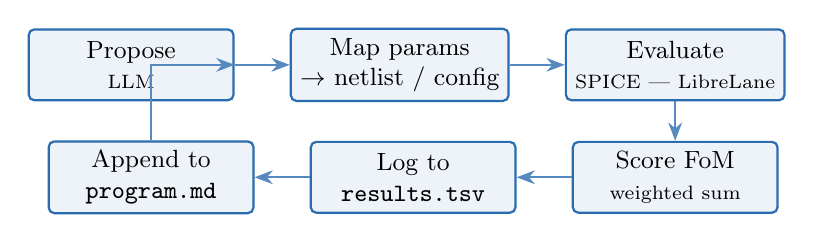
\begin{tikzpicture}[node distance=0.5cm and 0.7cm]
    \node[agent]  (prop) {Propose\\\scriptsize LLM};
    \node[agent, right=of prop] (map) {Map params\\$\rightarrow$ netlist / config};
    \node[agent, right=of map] (eval) {Evaluate\\\scriptsize SPICE | LibreLane};
    \node[agent, below=of eval] (fom) {Score FoM\\\scriptsize weighted sum};
    \node[agent, left=of fom] (log) {Log to\\\cmd{results.tsv}};
    \node[agent, left=of log] (prog) {Append to\\\cmd{program.md}};
    \draw[arrow] (prop) -- (map);
    \draw[arrow] (map) -- (eval);
    \draw[arrow] (eval) -- (fom);
    \draw[arrow] (fom) -- (log);
    \draw[arrow] (log) -- (prog);
    \draw[arrow] (prog) |- (prop);
  \end{tikzpicture}
  \end{center}
  \vspace{0.3em}
  \footnotesize
  \begin{itemize}
    \item Same loop for both domains; different \term{evaluator} and
          \term{design-space} plug-ins.
    \item \cmd{program.md} -- narrative log the LLM reads back on the
          next turn. Keeps context small.
    \item \cmd{results.tsv} -- numeric history; enables plot/resume.
    \item \cmd{budget} -- hard cap on iterations. Analog: tens.
          Digital: a handful.
  \end{itemize}
  \note{%
    This is the Karpathy-autoresearch pattern applied twice. Each loop
    iteration is a proposal, a mapping step (params $\rightarrow$ a
    deck or a config), an external evaluation, a score, and a log.\par
    Why persist to markdown + TSV? Two reasons: (1) it is human-readable
    so the user can inspect the run mid-flight, (2) the LLM can re-hydrate
    context by reading only \cmd{program.md} + the last few rows of
    \cmd{results.tsv}, instead of replaying the entire prompt history
    (context windows are expensive).\par
    Design-space shape is the big difference between the two loops:
    analog is continuous in W/L and bias (we snap to grid), digital is
    discrete over knob sets (density \cmd{\{60,65,70\}}, clock \cmd{\{50,40,30\}}).
    The runner handles both via a uniform \cmd{Parameter} interface.}
\end{frame}

\section{MCP + skills registry}

\begin{frame}[fragile]{MCP: making the stack portable}
  \cmd{eda-mcp} (stdio Model Context Protocol server) exposes the repo's
  primitives to any MCP-aware client (Claude Code, IDE extensions, custom
  tools):
  \begin{itemize}\footnotesize
    \item \term{Skills}: named prompts rendered from Markdown bundles
          (\cmd{analog.gmid\_sizing}, \cmd{digital.cocotb\_testbench},
          \cmd{flow.drc\_checker}, \ldots).
    \item \term{LUTs}: gm/ID tables for all registered PDK/device pairs.
    \item \term{Runners}: SPICE, LibreLane, DRC, LVS -- same code the
          agents call internally.
    \item \term{Topology registry}: list + metadata of circuit topologies.
  \end{itemize}
  \begin{lstlisting}[style=shellstyle]
# Register the server in ~/.config/claude-code/mcp.json
{"mcpServers": {"eda-agents": {"type": "stdio",
                "command": "eda-mcp"}}}
  \end{lstlisting}
  \footnotesize
  Full example: \cmd{src/eda\_agents/templates/mcp.json}.
  \note{%
    The MCP server is the integration seam. Without it, every consumer
    has to depend on the \cmd{eda\_agents} Python package and know the
    internal module layout. With it, the consumer asks for
    \cmd{get\_skill(\"analog.gmid\_sizing\")} or
    \cmd{run\_librelane(project\_dir, to=\"SIGNOFF\")} by name.\par
    Namespaces shipped today: \cmd{analog.*} (10+ skills),
    \cmd{digital.*} (cocotb TB authoring, RTL-to-GDS driver, etc.),
    \cmd{flow.*} (DRC checker, DRC fixer). The \cmd{list\_skills}
    tool enumerates them at runtime so an agent can discover what is
    available.\par
    LUT access is non-trivial: IHP SG13G2 LUTs live in an external
    \cmd{ihp-gmid-kit} clone; GF180 LUTs auto-download on first use and
    cache under \cmd{\char126/.cache/eda-agents/gmid\_luts/}. The MCP
    server hides all of that.}
\end{frame}

\section{Where to go next}

\begin{frame}{Starting points}
  \begin{itemize}\small
    \item \textbf{Run the analog loop:}
          \cmd{examples/07\_autoresearch\_circuit.py} -- Miller OTA
          sizing with SPICE feedback.
    \item \textbf{Run the digital loop:}
          \cmd{examples/09\_rtl2gds\_digital.py --backend cc\_cli}
          drives the 5-agent tree end-to-end on GF180 or IHP.
    \item \textbf{Tune LibreLane knobs:}
          \cmd{examples/10\_digital\_autoresearch.py} (greedy search).
    \item \textbf{Claude Code agent invocations:}
          \cmd{/agents gf180-docker-digital},
          \cmd{/agents analog-sizing-advisor},
          \cmd{/agents analog-topology-recommender}.
    \item \textbf{Hands-on tutorial:}
          \cmd{../rtl2gds-gf180-docker/demo/rtl2gds\_counter.ipynb} --
          4-bit counter, 8 notebook cells.
  \end{itemize}
  \vspace{0.6em}
  \footnotesize
  Source of truth for names + tool rosters:
  \cmd{.claude/agents/*.md}, \cmd{src/eda\_agents/agents/digital\_adk\_agents.py},
  \cmd{src/eda\_agents/skills/\{analog,digital\}.py}.
  \note{%
    Starter recipe for a new user: run the analog example first (it's
    fast, under 5 min on a laptop, and teaches the
    \cmd{program.md} / \cmd{results.tsv} convention); then try
    \cmd{09\_rtl2gds\_digital.py --dry-run} to see the agent flow
    without spending LLM tokens; then the counter notebook.\par
    For real work: invoke the Claude Code agent slash commands.
    \cmd{/agents gf180-docker-digital} hands you a Claude Code session
    with the toolchain, skills, and safety rails already wired in.
    Safer than copy-pasting prompts.}
\end{frame}

\begin{frame}{Thank you}
  \begin{center}
    \Large The agents are infrastructure, not magic.\\[0.4em]
    \normalsize Every tool they use is in the repo. Read the code.\\[0.8em]
    \small \cmd{github.com/Mauricio-xx/eda-agents}
  \end{center}
  \note{%
    Closing stance: resist the framing that ``AI does the design.''
    What actually happens is that humans encoded a design methodology
    (gm/ID for analog, the LibreLane flow for digital) as skills,
    topologies, and evaluators; the LLM drives the loop, but the loop
    is made of our code and our rules. Debugging an autoresearch run is
    reading \cmd{program.md} and \cmd{results.tsv}, not prompting
    harder.\par
    Invite questions on: adding a new topology, adding a new skill,
    wiring a new PDK, or integrating a custom evaluator.}
\end{frame}


\end{document}
